\clearpage
\section{The ablations in full}\label{app:abl-detail}

This appendix holds the detail behind \cref{sec:ablations}: the target families and the sources (\cref{app:abl-families}), and, for each group of parts, the refits of single cells that show how it acts (\cref{sec:abl-test,sec:abl-k3,sec:abl-smalln,sec:abl-label}), and the core in detail (\cref{app:core-detail}). Everything here is on the five ablation suites unless stated, and only \code{dlheld7} among them is held out.

% ------------------------------------------------------------------------------------------------------------------
\subsection{Families, sources and every target}\label{app:abl-families}

\paragraph{Pairing.} An ablation runs on DFG alone's training sets, column permutations and cross-validation folds: the training sets come from the target's and seed's own random stream, the column order and the folds from the fit's stream, and both streams are DFG alone's. Its $\nstar$ is compared with DFG alone's $\nstar$ computed from the same seeds of DFG alone's own runs.

\paragraph{Families.} Each target is assigned by hand, from its definition, to one of the nine groups of \cref{sec:interp-atlas} and to three classes (post hoc; \repo{study/part11/interp/ablations/families.py}). \emph{Character targets} are parities, staircases, multiplexers, compositions of parities and majorities and thresholds of a few characters, DNFs, CNFs, decision lists, read-once and random formulas: 71 of the 138 targets, 25 of the 65. \emph{Halfspaces} are majorities and thresholds of a weighted sum, with the dictator, $\mathrm{AND}(x_1,x_2,x_3)$ and an AND of two halfspaces (13 and 7). \emph{Symmetric and mixture targets} are functions of one signed sum, alone or with a parity, a gate, a second sum or an inner term (54 and 33). This class differs from the 54 sum-structured targets of \cref{sec:tasks} by two targets each way: it includes sym8 and sym9, and it counts f7\_01 and fd\_01, thresholds of an unsigned sum, as halfspaces. It keeps f7\_10, $[x_1+\dots+x_5+2x_6\le-1]$, among the mixtures, where the atlas puts it, although it is a threshold of a weighted sum. Counted as a halfspace, f7\_10 would move four class means by more than 0.05, all of them the halfspaces': under \code{strict}, \code{noblocks} and \code{labelnoise} from $-0.23$, $-0.19$ and $-0.17$ to $-0.17$, $-0.07$ and $-0.08$, and under \code{nosums} from $+0.05$ to $+0.11$ (\texttt{verification} in \repo{study/part11/interp/ablations/ablations.json}).

\paragraph{Sources.} The summaries are in \repo{study/part11/RESULTS.json} (\texttt{q5\_ablations}, \texttt{q5b\_core}), written by \repo{study/part11/compare_dfg.py}. The groupings, the nulls, the predictions of \cref{sec:abl-test} and the leave-one-in runs of \cref{sec:core} are in \repo{study/part11/interp/ablations/ablations.json}, written by \repo{study/part11/interp/ablations/ablations.py}; the analysis is \repo{study/part11/interp/ablations/ABLATIONS.md}. Models are read from refits of single cells (\repo{study/part11/interp/ablations/refit.py}). A refit uses the instrumented copy of \cref{sec:interp-calib}, so that every feature carries the class that admitted it: the class whose test gave it its largest $z_S$ in its round (\cref{sec:round}), so a character attributed to an extension or the local class may also pass that round's global test. All 38 refits of the analysis, and the 42 made when its verification was applied, reproduce their run's result file exactly in test error and FLOP count (\repo{study/part11/interp/ablations/results/refits.json}, \texttt{refits\_verif.json}). In four cells the same fit through the evaluation's own loader of the frozen file gives the same model, term by term (\repo{study/part11/interp/ablations/results/refit_crosscheck.json}). A term's s.d.\ is the standard deviation of its contribution on the test inputs, as in \cref{sec:interp-how}. An independent verifier checked the analysis, and its corrections are applied here (\repo{study/part11/interp/ablations/VERIFY_ABLATIONS.md}; \cref{app:interp-workflow}).

\paragraph{The paired null in full} \status{Numerical; post hoc}. On seed 0 the re-permuted fits move 1 of the 65 targets beyond $\pm0.25$ (dlist5, $+0.39$), and 10 of the 65 ratios are not zero; the mean $|\text{ratio}|$ is 0.012. On seeds 0 and 1 they move 3 (andxor $-0.69$, thrsum $-0.66$, h6\_07 $+0.40$), with mean $|\text{ratio}|$ 0.038. Over all 138 targets of the 11 suites they move 8 on seeds 0 and 1 (mean $|\text{ratio}|$ 0.040). The unpaired null moves 23 to 31 of the 65 targets, depending on the pair of seeds. Like for like, one seed against one, it moves 23 where the paired null moves 1, with mean $|\text{ratio}|$ 0.339 against 0.012: it overstates the noise of a paired comparison 20 to 30 times. Against the two-seed paired null, which is not like for like, its mean $|\text{ratio}|$ is 8.8 times as large (23 targets moved against 3).

\paragraph{Which targets move} \status{Numerical}. Under \code{nosums}, character targets lose little ($+0.16$; rand3, parmaj, h6\_05, fd\_07 and dnf3 move up). In the atlas, these are kinds of target that are encoded in part by blocks before their characters are all detectable: parmaj by two folded blocks, the formulas h6\_05, fd\_07 and dnf3 by the blocks of a clause or term, and random formulas such as rand3 by blocks on the inputs that follow their first characters (\cref{sec:interp-atlas}). Of the 15 targets \code{labelnoise} moves up, 9 are character targets, 6 of them formulas (family mean $+0.33$), and 6 are symmetric or mixture targets (mixtures $+0.15$). Of the 10 that \code{nosmalln} moves up, 8 are character targets (3 compositions, 3 formulas, par2 and rand2), with fd\_04 and sym7. Like for like, the mean $|\text{ratio}|$ of the two-seed runs, \code{noeig} and \code{nocomp}, is 0.026 and 0.043, against 0.038 for the paired null on two seeds; that of the one-seed runs, \code{noweighted}, \code{lsread} and \code{K3}, is 0.020, 0.032 and 0.075, against 0.012 on one seed. The per-family means are in \cref{tab:abl-family}, and every target's ratio in \cref{fig:ablations}.

\emph{Reading of the single changes, in full} \status{Heuristic}. On these suites DFG's results come from the sum blocks, with the residual scaling of the tests and the small-$n$ machinery as smaller contributors. As far as counts against one replicate of the null can tell, five parts can each be removed without a change larger than an arbitrary perturbation of the path produces: the eigenvector seeds, the composition classes, the weighted blocks, the logistic refinement and, but for one target (par4), the degree-4 search. Single targets still move further than any move of the null (h6\_10, par4, rand1). Two qualifications apply. The suites contain few targets that need those parts: one pure 4-parity, no dense halfspace on more than 13 inputs, no degree-5 parity. And the parts are removed one at a time, so they may substitute for one another. \Cref{sec:core} removes them together.

\begin{figure}[t]
\centering
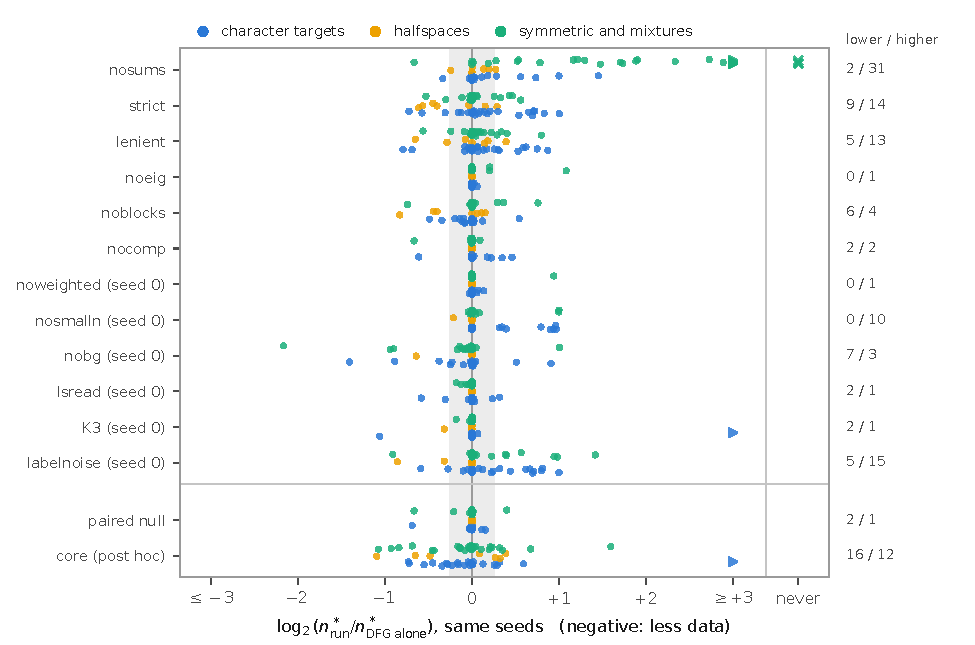
\includegraphics[width=\linewidth]{figures/fig_ablations.pdf}
\caption{The 62 targets of the five ablation suites that DFG alone learns, one row per run: the $\log_2$ ratio of the run's $\nstar$ to DFG alone's on the same seeds \status{Numerical}. Colour gives the target's class; the grey band is the tie band $\pm0.25$. Ratios beyond $\pm3$ are drawn at the edge (triangles), and ``never'' (the run never reaches 10\% error where DFG alone does) in the right-hand column. Right: the numbers of targets clearly lower / clearly higher. Bottom: the paired null on seeds 0 and 1 (post hoc) and the core DFG of \cref{sec:core} on the same 65 targets (post hoc). Source: \repo{study/part11/interp/ablations/ablations.json} via \repo{paper_dfg/make_figures.py}; the plotted points are in \repo{paper_dfg/figures/fig_ablations.json}.}
\label{fig:ablations}
\end{figure}

\begin{table}[t]
\centering{\footnotesize\setlength{\tabcolsep}{3pt}\renewcommand{\arraystretch}{1.05}
\begin{tabular}{@{}lcccccccc@{}}
\toprule
run & \hd{parities\\(3)} & \hd{stair-\\cases\\(1)} & \hd{half-\\spaces\\(7)} & \hd{compo-\\sitions\\(6)} & \hd{formulas\\(11)} & \hd{random\\formulas\\(4)} & \hd{sym-\\metric\\(12)} & \hd{mixtures\\(21)}\\
\midrule
\code{nosums} & \begin{tabular}[t]{@{}c@{}}$+0.00$\\{\scriptsize (0/0)}\end{tabular} & \begin{tabular}[t]{@{}c@{}}$+0.00$\\{\scriptsize (0/0)}\end{tabular} & \begin{tabular}[t]{@{}c@{}}$+0.05$\\{\scriptsize (0/1)}\end{tabular} & \begin{tabular}[t]{@{}c@{}}$+0.11$\\{\scriptsize (1/1)}\end{tabular} & \begin{tabular}[t]{@{}c@{}}$+0.17$\\{\scriptsize (0/3)}\end{tabular} & \begin{tabular}[t]{@{}c@{}}$+0.36$\\{\scriptsize (0/1)}\end{tabular} & \begin{tabular}[t]{@{}c@{}}$+2.78$\\{\scriptsize (0/9)}\end{tabular} & \begin{tabular}[t]{@{}c@{}}$+1.54$\\{\scriptsize (1/16)}\end{tabular}\\
\code{strict} & \begin{tabular}[t]{@{}c@{}}$+0.40$\\{\scriptsize (0/1)}\end{tabular} & \begin{tabular}[t]{@{}c@{}}$+0.83$\\{\scriptsize (0/1)}\end{tabular} & \begin{tabular}[t]{@{}c@{}}$-0.23$\\{\scriptsize (4/1)}\end{tabular} & \begin{tabular}[t]{@{}c@{}}$+0.09$\\{\scriptsize (2/2)}\end{tabular} & \begin{tabular}[t]{@{}c@{}}$+0.01$\\{\scriptsize (1/2)}\end{tabular} & \begin{tabular}[t]{@{}c@{}}$+0.39$\\{\scriptsize (0/2)}\end{tabular} & \begin{tabular}[t]{@{}c@{}}$-0.01$\\{\scriptsize (0/0)}\end{tabular} & \begin{tabular}[t]{@{}c@{}}$+0.06$\\{\scriptsize (2/5)}\end{tabular}\\
\code{lenient} & \begin{tabular}[t]{@{}c@{}}$-0.26$\\{\scriptsize (1/0)}\end{tabular} & \begin{tabular}[t]{@{}c@{}}$+0.00$\\{\scriptsize (0/0)}\end{tabular} & \begin{tabular}[t]{@{}c@{}}$-0.04$\\{\scriptsize (2/1)}\end{tabular} & \begin{tabular}[t]{@{}c@{}}$+0.36$\\{\scriptsize (0/3)}\end{tabular} & \begin{tabular}[t]{@{}c@{}}$+0.19$\\{\scriptsize (0/5)}\end{tabular} & \begin{tabular}[t]{@{}c@{}}$-0.11$\\{\scriptsize (1/0)}\end{tabular} & \begin{tabular}[t]{@{}c@{}}$+0.07$\\{\scriptsize (0/1)}\end{tabular} & \begin{tabular}[t]{@{}c@{}}$+0.05$\\{\scriptsize (1/3)}\end{tabular}\\
\code{noeig} & \begin{tabular}[t]{@{}c@{}}$+0.00$\\{\scriptsize (0/0)}\end{tabular} & \begin{tabular}[t]{@{}c@{}}$+0.00$\\{\scriptsize (0/0)}\end{tabular} & \begin{tabular}[t]{@{}c@{}}$+0.00$\\{\scriptsize (0/0)}\end{tabular} & \begin{tabular}[t]{@{}c@{}}$+0.00$\\{\scriptsize (0/0)}\end{tabular} & \begin{tabular}[t]{@{}c@{}}$+0.01$\\{\scriptsize (0/0)}\end{tabular} & \begin{tabular}[t]{@{}c@{}}$-0.00$\\{\scriptsize (0/0)}\end{tabular} & \begin{tabular}[t]{@{}c@{}}$+0.02$\\{\scriptsize (0/0)}\end{tabular} & \begin{tabular}[t]{@{}c@{}}$+0.06$\\{\scriptsize (0/1)}\end{tabular}\\
\code{noblocks} & \begin{tabular}[t]{@{}c@{}}$+0.00$\\{\scriptsize (0/0)}\end{tabular} & \begin{tabular}[t]{@{}c@{}}$+0.00$\\{\scriptsize (0/0)}\end{tabular} & \begin{tabular}[t]{@{}c@{}}$-0.19$\\{\scriptsize (3/0)}\end{tabular} & \begin{tabular}[t]{@{}c@{}}$-0.07$\\{\scriptsize (1/0)}\end{tabular} & \begin{tabular}[t]{@{}c@{}}$+0.01$\\{\scriptsize (0/1)}\end{tabular} & \begin{tabular}[t]{@{}c@{}}$-0.12$\\{\scriptsize (1/0)}\end{tabular} & \begin{tabular}[t]{@{}c@{}}$-0.00$\\{\scriptsize (0/0)}\end{tabular} & \begin{tabular}[t]{@{}c@{}}$+0.04$\\{\scriptsize (1/3)}\end{tabular}\\
\code{nocomp} & \begin{tabular}[t]{@{}c@{}}$+0.00$\\{\scriptsize (0/0)}\end{tabular} & \begin{tabular}[t]{@{}c@{}}$+0.00$\\{\scriptsize (0/0)}\end{tabular} & \begin{tabular}[t]{@{}c@{}}$+0.00$\\{\scriptsize (0/0)}\end{tabular} & \begin{tabular}[t]{@{}c@{}}$-0.07$\\{\scriptsize (1/0)}\end{tabular} & \begin{tabular}[t]{@{}c@{}}$+0.08$\\{\scriptsize (0/2)}\end{tabular} & \begin{tabular}[t]{@{}c@{}}$+0.05$\\{\scriptsize (0/0)}\end{tabular} & \begin{tabular}[t]{@{}c@{}}$+0.00$\\{\scriptsize (0/0)}\end{tabular} & \begin{tabular}[t]{@{}c@{}}$-0.03$\\{\scriptsize (1/0)}\end{tabular}\\
\code{noweighted} & \begin{tabular}[t]{@{}c@{}}$+0.00$\\{\scriptsize (0/0)}\end{tabular} & \begin{tabular}[t]{@{}c@{}}$+0.00$\\{\scriptsize (0/0)}\end{tabular} & \begin{tabular}[t]{@{}c@{}}$+0.00$\\{\scriptsize (0/0)}\end{tabular} & \begin{tabular}[t]{@{}c@{}}$+0.00$\\{\scriptsize (0/0)}\end{tabular} & \begin{tabular}[t]{@{}c@{}}$+0.02$\\{\scriptsize (0/0)}\end{tabular} & \begin{tabular}[t]{@{}c@{}}$+0.00$\\{\scriptsize (0/0)}\end{tabular} & \begin{tabular}[t]{@{}c@{}}$+0.00$\\{\scriptsize (0/0)}\end{tabular} & \begin{tabular}[t]{@{}c@{}}$+0.04$\\{\scriptsize (0/1)}\end{tabular}\\
\code{nosmalln} & \begin{tabular}[t]{@{}c@{}}$+0.26$\\{\scriptsize (0/1)}\end{tabular} & \begin{tabular}[t]{@{}c@{}}$+0.00$\\{\scriptsize (0/0)}\end{tabular} & \begin{tabular}[t]{@{}c@{}}$-0.03$\\{\scriptsize (0/0)}\end{tabular} & \begin{tabular}[t]{@{}c@{}}$+0.38$\\{\scriptsize (0/3)}\end{tabular} & \begin{tabular}[t]{@{}c@{}}$+0.15$\\{\scriptsize (0/3)}\end{tabular} & \begin{tabular}[t]{@{}c@{}}$+0.22$\\{\scriptsize (0/1)}\end{tabular} & \begin{tabular}[t]{@{}c@{}}$+0.11$\\{\scriptsize (0/1)}\end{tabular} & \begin{tabular}[t]{@{}c@{}}$+0.05$\\{\scriptsize (0/1)}\end{tabular}\\
\code{nobg} & \begin{tabular}[t]{@{}c@{}}$+0.00$\\{\scriptsize (0/0)}\end{tabular} & \begin{tabular}[t]{@{}c@{}}$+0.04$\\{\scriptsize (0/0)}\end{tabular} & \begin{tabular}[t]{@{}c@{}}$-0.09$\\{\scriptsize (1/0)}\end{tabular} & \begin{tabular}[t]{@{}c@{}}$-0.12$\\{\scriptsize (1/0)}\end{tabular} & \begin{tabular}[t]{@{}c@{}}$-0.10$\\{\scriptsize (1/1)}\end{tabular} & \begin{tabular}[t]{@{}c@{}}$+0.00$\\{\scriptsize (1/1)}\end{tabular} & \begin{tabular}[t]{@{}c@{}}$-0.04$\\{\scriptsize (0/0)}\end{tabular} & \begin{tabular}[t]{@{}c@{}}$-0.16$\\{\scriptsize (3/1)}\end{tabular}\\
\code{lsread} & \begin{tabular}[t]{@{}c@{}}$+0.00$\\{\scriptsize (0/0)}\end{tabular} & \begin{tabular}[t]{@{}c@{}}$+0.00$\\{\scriptsize (0/0)}\end{tabular} & \begin{tabular}[t]{@{}c@{}}$+0.00$\\{\scriptsize (0/0)}\end{tabular} & \begin{tabular}[t]{@{}c@{}}$+0.06$\\{\scriptsize (0/1)}\end{tabular} & \begin{tabular}[t]{@{}c@{}}$-0.06$\\{\scriptsize (2/0)}\end{tabular} & \begin{tabular}[t]{@{}c@{}}$-0.01$\\{\scriptsize (0/0)}\end{tabular} & \begin{tabular}[t]{@{}c@{}}$-0.00$\\{\scriptsize (0/0)}\end{tabular} & \begin{tabular}[t]{@{}c@{}}$-0.02$\\{\scriptsize (0/0)}\end{tabular}\\
\code{K3} & \begin{tabular}[t]{@{}c@{}}$+1.00$\\{\scriptsize (0/1)}\end{tabular} & \begin{tabular}[t]{@{}c@{}}$+0.07$\\{\scriptsize (0/0)}\end{tabular} & \begin{tabular}[t]{@{}c@{}}$-0.05$\\{\scriptsize (1/0)}\end{tabular} & \begin{tabular}[t]{@{}c@{}}$+0.00$\\{\scriptsize (0/0)}\end{tabular} & \begin{tabular}[t]{@{}c@{}}$-0.00$\\{\scriptsize (0/0)}\end{tabular} & \begin{tabular}[t]{@{}c@{}}$-0.26$\\{\scriptsize (1/0)}\end{tabular} & \begin{tabular}[t]{@{}c@{}}$+0.00$\\{\scriptsize (0/0)}\end{tabular} & \begin{tabular}[t]{@{}c@{}}$-0.01$\\{\scriptsize (0/0)}\end{tabular}\\
\code{labelnoise} & \begin{tabular}[t]{@{}c@{}}$+0.00$\\{\scriptsize (0/0)}\end{tabular} & \begin{tabular}[t]{@{}c@{}}$+0.70$\\{\scriptsize (0/1)}\end{tabular} & \begin{tabular}[t]{@{}c@{}}$-0.17$\\{\scriptsize (2/0)}\end{tabular} & \begin{tabular}[t]{@{}c@{}}$+0.11$\\{\scriptsize (1/1)}\end{tabular} & \begin{tabular}[t]{@{}c@{}}$+0.33$\\{\scriptsize (1/6)}\end{tabular} & \begin{tabular}[t]{@{}c@{}}$+0.19$\\{\scriptsize (0/1)}\end{tabular} & \begin{tabular}[t]{@{}c@{}}$+0.10$\\{\scriptsize (0/1)}\end{tabular} & \begin{tabular}[t]{@{}c@{}}$+0.15$\\{\scriptsize (1/5)}\end{tabular}\\
\midrule
paired null (0, 1) & \begin{tabular}[t]{@{}c@{}}$-0.00$\\{\scriptsize (0/0)}\end{tabular} & \begin{tabular}[t]{@{}c@{}}$+0.00$\\{\scriptsize (0/0)}\end{tabular} & \begin{tabular}[t]{@{}c@{}}$+0.00$\\{\scriptsize (0/0)}\end{tabular} & \begin{tabular}[t]{@{}c@{}}$-0.11$\\{\scriptsize (1/0)}\end{tabular} & \begin{tabular}[t]{@{}c@{}}$+0.02$\\{\scriptsize (0/0)}\end{tabular} & \begin{tabular}[t]{@{}c@{}}$-0.00$\\{\scriptsize (0/0)}\end{tabular} & \begin{tabular}[t]{@{}c@{}}$-0.02$\\{\scriptsize (0/0)}\end{tabular} & \begin{tabular}[t]{@{}c@{}}$-0.01$\\{\scriptsize (1/1)}\end{tabular}\\
paired null (0) & \begin{tabular}[t]{@{}c@{}}$-0.00$\\{\scriptsize (0/0)}\end{tabular} & \begin{tabular}[t]{@{}c@{}}$+0.00$\\{\scriptsize (0/0)}\end{tabular} & \begin{tabular}[t]{@{}c@{}}$+0.00$\\{\scriptsize (0/0)}\end{tabular} & \begin{tabular}[t]{@{}c@{}}$-0.02$\\{\scriptsize (0/0)}\end{tabular} & \begin{tabular}[t]{@{}c@{}}$+0.02$\\{\scriptsize (0/1)}\end{tabular} & \begin{tabular}[t]{@{}c@{}}$-0.00$\\{\scriptsize (0/0)}\end{tabular} & \begin{tabular}[t]{@{}c@{}}$+0.00$\\{\scriptsize (0/0)}\end{tabular} & \begin{tabular}[t]{@{}c@{}}$-0.00$\\{\scriptsize (0/0)}\end{tabular}\\
unpaired null & \begin{tabular}[t]{@{}c@{}}$-0.33$\\{\scriptsize (1/0)}\end{tabular} & \begin{tabular}[t]{@{}c@{}}$+0.01$\\{\scriptsize (0/0)}\end{tabular} & \begin{tabular}[t]{@{}c@{}}$-0.17$\\{\scriptsize (2/1)}\end{tabular} & \begin{tabular}[t]{@{}c@{}}$+0.17$\\{\scriptsize (1/2)}\end{tabular} & \begin{tabular}[t]{@{}c@{}}$-0.01$\\{\scriptsize (2/1)}\end{tabular} & \begin{tabular}[t]{@{}c@{}}$-0.07$\\{\scriptsize (1/1)}\end{tabular} & \begin{tabular}[t]{@{}c@{}}$+0.01$\\{\scriptsize (1/1)}\end{tabular} & \begin{tabular}[t]{@{}c@{}}$-0.06$\\{\scriptsize (5/4)}\end{tabular}\\
\midrule
core (post hoc) & \begin{tabular}[t]{@{}c@{}}$+2.01$\\{\scriptsize (0/1)}\end{tabular} & \begin{tabular}[t]{@{}c@{}}$-0.08$\\{\scriptsize (0/0)}\end{tabular} & \begin{tabular}[t]{@{}c@{}}$-0.17$\\{\scriptsize (3/3)}\end{tabular} & \begin{tabular}[t]{@{}c@{}}$-0.15$\\{\scriptsize (3/1)}\end{tabular} & \begin{tabular}[t]{@{}c@{}}$-0.04$\\{\scriptsize (2/2)}\end{tabular} & \begin{tabular}[t]{@{}c@{}}$-0.27$\\{\scriptsize (2/1)}\end{tabular} & \begin{tabular}[t]{@{}c@{}}$-0.03$\\{\scriptsize (0/0)}\end{tabular} & \begin{tabular}[t]{@{}c@{}}$-0.05$\\{\scriptsize (6/4)}\end{tabular}\\
\bottomrule
\end{tabular}
}
\caption{The ablations by target family (the groups of \cref{sec:interp-atlas}; group sizes in the header) on the 65 targets of the five ablation suites \status{Numerical; families post hoc}. Eight of the nine groups appear: no target of the multiplexer group (mux6, mux11) is in these suites, and \code{designed}'s mux is grouped with the compositions. Each cell: mean $\log_2$ ratio over the targets both learn, and the targets clearly lower / clearly higher. The symmetric group holds the three targets that neither DFG alone nor any ablation learns (fd\_10, h6\_00, f7\_05), so its means are over 9 targets (6 under \code{nosums}). Bottom: the paired and unpaired nulls, and the core DFG on the same 65 targets (post hoc). Source: \repo{study/part11/interp/ablations/ablations.json}.}
\label{tab:abl-family}
\end{table}

% ------------------------------------------------------------------------------------------------------------------
\subsection{The test or the search: the refits}\label{sec:abl-test}

\code{strict} ($\delta=10^{-4}$) and \code{lenient} ($\delta=0.9$) move the log term of every test by $+6.91$ and $-2.20$ nats. If a target's data cost is set by a test, its $\nstar$ should move by a predictable amount; if it is set by the search, it should not move. \Cref{sec:interp-when} goes through these two runs target by target (\cref{fig:dyn-when}); this subsection gives the predictions in detail and the refits behind the asymmetry between the two.

\paragraph{Parities: the test, exactly} \status{Numerical}. By \cref{prop:parity}, a $k$-parity passes round 0's test exactly when $n(1-\bar y^2)>n_{\rm thr}(k,d)$, and $n_{\rm thr}$ moves by $+13.8$ and $-4.4$ rows with $\delta$. At $d=30$ it moves from 22.3, 26.8 and 30.6 ($k=2,3,4$) to 36.1, 40.6 and 44.4 under \code{strict}, and to 17.9, 22.4 and 26.2 under \code{lenient}. Applied seed by seed to each training set's own $\bar y$ (post hoc: error 0 where the test passes, DFG alone's error but at least 0.45 where it fails, DFG alone's measured cell at $n=16$), this predicts the measured changes of $\nstar$ to within 0.03: par3 $+0.98$ against $+1.00$ under \code{strict}, and 0 against 0 under \code{lenient}; par4 $+0.20$ against $+0.21$, and $-0.79$ against $-0.79$. par2 moves under neither, because the forced variant fits it at $n=16$, below every $n_{\rm thr}$ here. The cross-validation's choice at $n=16$ can depend on $\delta$ (par4, seed 1, keeps the forced variant only under \code{lenient}), but every $n=16$ cell stays near error 0.5, or 0 for par2, so $\nstar$ does not move.

\paragraph{Other character targets} \status{Numerical}. By \cref{prop:nglob}(b), $n_{\rm glob}$ is proportional to the log term, so \code{strict} should raise it by $+0.54$ to $+0.86$ doublings (degree 4 to degree 1), and \code{lenient} lower it by $-0.22$ to $-0.43$. \code{strict} raises $\nstar$ beyond 0.25 on 8 of the 25 character targets (par3, stair5, rand3, rand2, majpar, sparsepoly, h6\_03, h6\_05), and for 7 of them the first grid point at 10\% error (seed mean) moves one step; h6\_05's $\nstar$ moves within the same grid interval. \code{lenient} is not the mirror image: it lowers $\nstar$ on 2 targets (par4, rand2) and raises it on 8 (andxor, majpar, fd\_00, mux, fd\_07, dlist5, h6\_05, f7\_02). Two things go with the asymmetry. These targets are first fitted at $n=32$--256 (8 of their 16 seed cells at 32--64), and in 11 of the 16 by the forced variant. And of the tests that run below $n=120$, the one a more lenient $\delta$ moves most is the linear block's, whose threshold on 30 inputs (\cref{eq:lintest}) is 51.2 at $\delta=0.1$, 33.8 at $0.9$ and 81.7 at $10^{-4}$: \code{lenient} lowers it by a factor 0.66, against 0.74 for a degree-1 character, while \code{strict} raises it by 1.59, against 1.81. (The spectral edge, which runs from $n=4d=120$ on, moves more: the $n$ at which a fixed eigenvalue clears it scales by 0.61 and 1.64.) Refitted at those 16 first fits, the linear block enters under $\delta=0.9$ in 8 cells where it did not under $\delta=0.1$, and the cross-validation's choice of variant changes in 7; andxor and f7\_02 move through that choice alone (\repo{study/part11/interp/ablations/results/lenient_first_fits.json}). Two refits show the mechanisms.
\begin{itemize}
\item \emph{majpar at $n=64$} (seed 0). With $\delta=0.1$ nothing passes in round 0. The forced variant adds $\chi_{\{1,2\}}$ and then $\chi_{\{3,4\}}$, and $\chi_{\{5,6\}}$ passes its own test in round 2: error 0.067. With $\delta=0.9$, $\chi_{\{1,2\}}$ passes in round 0 and the linear block enters with 30 degree-1 characters, none of them in majpar's Fourier support. In round 1 $\chi_{\{3,4\}}$ passes its test, but the constant, $\chi_{\{1,2\}}$ and the 30 linear characters already fill the $n/2=32$ features that least squares allows, so the fit stops, with error 0.341. This is a second cost of the linear block at small $n$: its characters take the room a later character needs. With $\delta=10^{-4}$ the forced pairs are the same, but $\chi_{\{5,6\}}$ fails its test: error 0.269.
\item \emph{f7\_02 at $n=128$} (a DNF of three terms, seed 1), the other direction: the one formula on which \code{strict} lowers $\nstar$ (it also lowers andxor and mux, two compositions that were not refitted). With $\delta=0.1$ the linear block enters, and the default variant is kept: error 0.202. With $\delta=10^{-4}$ nothing passes. The forced variant guesses the blocks $(x_2-x_6-x_8)$ and $(-x_3+x_5+x_7)$, two of the DNF's terms; the third term's block then passes its test, and the cross-validation keeps the forced variant: error 0.
\end{itemize}

\paragraph{Halfspaces and sum targets} \status{Numerical}. Halfspaces gain from a stricter test ($-0.23$; 4 of 7 lower). On f7\_01 at $n=128$, a degree-1 character that passes its own test first takes part of the exact block's signal in the block's second test, and with $\delta=10^{-4}$ the block enters instead (\cref{sec:interp-when}). On the 33 symmetric and mixture targets the class means are $+0.04$ and $+0.05$ (30 learned; 5 and 4 higher, 2 and 1 lower). At the true block's detection point $n_{\rm detect}$ (Part 10's block statistics on seed 0's rows, re-thresholded post hoc for each $\delta$; approximate for the modulated blocks, whose statistic was stored only as a ratio to its threshold), \code{strict} moves the block threshold by $+0.20$ to $+0.30$ doublings of $n$. The ablation analysis uses Part 10's round-0 detection points; with the points Part 10's verifier corrected for the gate and multiplexer mixtures (\cref{tab:dyn-when}), f7\_03's $\nstar$ lies below its detection point. On the 6 targets whose $\nstar$ lies a doubling or more beyond $n_{\rm detect}$ (7 with the uncorrected points), \code{strict} changes $\nstar$ by at most 0.05. On the other 24, $\nstar$ lies less than a doubling beyond $n_{\rm detect}$ (for 20 at or below it; 23 and 18 with the uncorrected points), and the grid cannot separate the test from the search (\repo{paper_dfg/tables/interp_numbers.json}, \texttt{fig\_dyn\_when.gap\_split}).

% ------------------------------------------------------------------------------------------------------------------
\subsection{Degree 4 without the degree-4 search}\label{sec:abl-k3}

\code{K3} sets $K=K_{\rm hi}=3$: the global search stops at degree 3, and the degree-5/6 search is off. $K$ also enters the union bound of every character class through $\ln(4KN/\delta)$ (\cref{eq:chartest}) and that of the sum-block test through $L_B$ (\cref{eq:blocktest}), so these tests become 0.29 nats more lenient. The linear block's test and the spectral edge use $\ln(1/\delta)$ only (\cref{eq:lintest,eq:spectest}) and do not change. On the 65 targets \code{K3} moves 3 (\cref{tab:ablations}).

\paragraph{par4} \status{Numerical; refits, seed 0}. Under \code{K3}, par4's test error is 0.49--0.50 at $n\le256$, 0 at 512, 0.50 at 1024, 0 at 2048 and 4096, and 0.49--0.50 at 8192 and 16384. In the three fitted cells the model's main term is a folded block on the parity's four inputs, admitted in round 0 by an additive block search: $|{-x_1}-x_2-x_3-x_4|$ at 512, $|x_1-x_2+x_3+x_4|$ at 2048 and $|x_1-x_2-x_3+x_4|$ at 4096, at 9.0, 34.5 and 70.9 times its threshold. Next to it the model holds an admitted product block: $|{-x_1}-x_2-x_3-x_4|\times|x_5-x_{14}|$ at 512 (term s.d.\ 0.40, against the folded block's 0.61), and split products at 2048 and 4096 (term s.d.\ 0.09 and 0.06). A $k$-parity is a function of any signed sum of its $k$ inputs, so one folded block represents it exactly (\cref{prop:blocks}). In the six empty cells from $n=64$ on (64, 128, 256, 1024, 8192 and 16384) the round-0 block searches' best candidates stand at 0.13--0.45 of their thresholds, and the model is the constant and the background. Yet the true folded block would pass at every $n\ge64$: on the round-0 residual a block that determines the labels has $T_B=n$ exactly, against a threshold of 56.9. The search finds it at 3 of these 9 grid sizes. With the degree-4 search, $\chi_{\{1,2,3,4\}}$ passes its round-0 test from $n=64$ on (\cref{prop:parity}).

\paragraph{mux and andxor} \status{Numerical; refits, seed 0}. These two targets have degree-4 coefficients of 0.75 and 0.5. Their test error under \code{K3} equals DFG alone's at every $n$, but the models differ.
\begin{itemize}
\item mux at $n=256$: DFG alone's largest term is $\chi_{\{1,2,3,4\}}$ (term s.d.\ 0.51), admitted by the degree-4 test in round 0. \code{K3} holds no degree-4 character; it has the blocks $(-x_1-x_2-x_3+x_4)$ and $(x_1+x_2+x_3+3x_4)$, and $\chi_{\{1,2,3\}}$, which the two-input extension of $\chi_{\{1\}}$ scores highest but the global degree-3 test of the same round also passes.
\item andxor at $n=256$: DFG alone holds its exact expansion $\chi_{\{1,2\}}$, $\chi_{\{3,4\}}$, $\chi_{\{1,2,3,4\}}$. \code{K3} holds the two pair characters and the weighted block $(x_1+x_2-3x_3x_4)$.
\end{itemize}

\paragraph{rand1, $-1.06$} \status{Numerical; refit, seed 0, $n=64$}. rand1 has 5 relevant inputs, $x_1$, $x_3$, $x_4$, $x_5$ and $x_6$, and degree-1 weight on 3 of them ($\pm0.375$ on $x_1$, $x_3$ and $x_5$). With $K=4$, round 0 admits the linear block (30 degree-1 characters), and the forced variant then guesses $\chi_{\{4,12,17\}}$: error 0.412. With $K=3$, $\chi_{\{1\}}$ passes its own, slightly more lenient test, so the linear block does not enter. The forced guess is then $\chi_{\{1,4,6\}}$, the local class adds $\chi_{\{4,6\}}$, and a block $(x_3-x_5)$ follows: error 0. This difference comes from $K$ in the union bound, not from the degree-4 search.

\emph{Reading} \status{Heuristic}. The degree-4 search is redundant where a target's degree-4 characters share their inputs with lower-degree structure: blocks on those inputs, and lower-degree characters, reach them. (In the refits of mux, the characters attributed to the extension and local classes also pass the global tests, so these refits do not show that those classes are needed.) It is indispensable for a degree-4 parity with no lower-degree footprint. The block test would admit the exact block from small $n$ on, but the block search starts from degree-1 and degree-2 statistics (\cref{prop:blocks}), which are zero for such a parity, so it finds the four inputs only by chance. The ablation suites contain one such target. \Cref{sec:core} adds three more.

% ------------------------------------------------------------------------------------------------------------------
\subsection{The small-\texorpdfstring{$n$}{n} machinery and the background}\label{sec:abl-smalln}

The atlas computed two counterfactuals on its 37 targets (\cref{sec:interp-atlas}): the variant DFG's cross-validation did not choose, refitted on the same rows, and each fitted model without its kernel background. \code{nosmalln} and \code{nobg} run them as learners, and on the 21 targets the ablation suites share with the atlas the two agree in 126 of 126 and 224 of 231 cells.

\paragraph{No forced variant, no cross-validation} \status{Numerical}. \code{nosmalln} fits the default variant on all $n$ rows. At $d=30$ it can differ from the atlas's ``always default'' refit only in the degree-5/6 subsample sizes (\cref{prop:compute}). Its seed-0 test error equals that refit's in all 126 cells with $n\le512$. Over the 65 targets, the mean test error rises by 0.012, 0.007, 0.022, 0.009 and 0.004 at $n=16$, 32, 64, 128 and 256, and by nothing from 512 on. $\nstar$ rises on 10 targets and falls on none (mean $+0.12$). Since \code{nosmalln} is the default variant, every cell where DFG alone does better is one where DFG alone kept the forced variant. The first fits lost this way are par2 and rand2 at $n=16$, majpar at 32 and 64, mux and sym7 at 64, fd\_04 at 128 and f7\_02 at 256. Each comes back one grid step later. Over the atlas's 222 cells, DFG's choice of variant is compared with the alternatives in \cref{app:interp-fits}.

\paragraph{No kernel background} \status{Numerical}. The background is added after the weights are fitted. A fitted model without it therefore gives exactly DFG's prediction without it for the same variant. The ablation can differ from that only where the cross-validation chooses another variant, because the fold fits lose their background too. \code{nobg}'s seed-0 error equals the atlas's model-without-background error in 224 of 231 cells. The other 7 are all at $n\le128$, so in each of them the choice changed. One is refitted: f7\_11 at $n=16$. DFG alone keeps the default variant there (held-out errors 6 and 3), the constant plus the background, with test error 0.301. Without the background, the default variant's held-out errors rise to 13, the forced variant is kept, and its model $\chi_{\{11\}}$, $\chi_{\{8\}}$ has error 0.077. Over the 65 targets the mean error rises by 0.015 and 0.016 at $n=16$ and 32, and falls by 0.009, 0.002, 0.003 and 0.002 at 64, 128, 256 and 512. $\nstar$ falls on 7 targets and rises on 3 (mean $-0.10$); f7\_11 falls most ($-2.17$).

\emph{Reading} \status{Heuristic}. With nothing else in the model, at $n=16$--32, the background is a Hebbian classifier, and it helps targets with a strong degree-1 part. From $n=64$ on it adds the noise of 30 residual correlations to a model that already fits. Through the cross-validation it can also make the default variant look better than it is, so that the forced variant's right guesses are kept less often (the 7 cells in which \code{nobg}'s choice of variant changed, such as f7\_11 at $n=16$), or worse (sym8 at $n=64$; \cref{sec:core}). Most $\nstar$ lie at 64--512, so the background costs data on balance on these suites.

% ------------------------------------------------------------------------------------------------------------------
% ------------------------------------------------------------------------------------------------------------------
\subsection{Tests scaled to the residual}\label{sec:abl-label}

\code{labelnoise} replaces $s$ by 1 in every test, so the tests are scaled to the labels' noise instead of the residual's: the character thresholds and the spectral edge, which are proportional to $s$, rise by the factor $1/s$, and the statistics of the blocks and of the linear block, which are divided by $s^2$, fall by the factor $s^2$. (The subsampled searches keep their subsample's root mean square, and a block's second test, on the projected residual, keeps that residual's variance.) In round 0 the residual is $y-\bar y$, with variance $1-\bar y^2$, and after the first features fit it shrinks. By \cref{prop:nglob}(c), characters admitted after round 0 enter 1.4--3.7 doublings below $n_{\rm glob}$ (class medians), mainly because the residual variance there is 3.2--19 times smaller (class medians; \cref{prop:nglob}, ``Checks'').

\paragraph{Results} \status{Numerical}. The mean ratio is $+0.14$ (15 higher, 5 lower). By family: formulas $+0.33$ (6 of 11 higher), the staircase $+0.70$, random formulas $+0.19$, mixtures $+0.15$ (5 of 21), compositions $+0.11$, symmetric targets $+0.10$, parities 0, halfspaces $-0.17$ (\cref{tab:abl-family}). The mean test error rises by 0.024 at $n=128$ (18 targets higher by more than 0.02, 2 lower) and by 0.013 at 256, and by at most 0.004 in absolute value elsewhere. Two refits at $n=128$ (seed 0) show the two ways the scaling matters.
\begin{itemize}
\item \emph{Later rounds}, rand3. DFG alone admits $\chi_{\{5,6\}}$ in round 0 ($s=1.00$), $\chi_{\{4,5,6\}}$ by the one-input extension in round 1 ($s=0.84$), $\chi_{\{5\}}$ and $\chi_{\{4,5\}}$ in round 2 ($s=0.77$; the local class scores both highest, and the global degree-1 test also passes $\chi_{\{5\}}$), and five modulated blocks and a spectral feature in rounds 3 and 4: error 0.049. With $s=1$ the first round is the same, but nothing passes in round 1, and the fit stops: error 0.317.
\item \emph{Biased labels}, far9 $=[|x_1+\dots+x_9|\ge5]$, whose round-0 residual has $s=0.71$. DFG alone admits the folded block $|x_1+\dots+x_9|$ and a spectral feature in round 0: error 0.006. With $s=1$ the character and spectral thresholds are 1.41 times higher, and the block search's statistic is divided by 1 instead of $s^2=0.51$, so the folded block falls from 1.52 to 0.77 times its threshold. Nothing passes, and the model is the constant and the background: error 0.181.
\end{itemize}

\emph{Reading} \status{Heuristic}. The residual scaling is what makes the growth greedy in the sense of DFG's design: each round's tests are calibrated to the noise left after the previous round, so weaker features pass once stronger ones are in. Its cost on these targets is modest, because the features that bring most targets below 10\% error enter in round 0 (\cref{sec:interp-order}). It is larger for formulas and staircases, whose later characters build on the first ones, and for targets with biased labels.

% ------------------------------------------------------------------------------------------------------------------
\subsection{The core in detail}\label{app:core-detail}

The core's code is the frozen file, with the constructor arguments \code{readout="ls"}, \code{sum_inner=False}, \code{sum_seeds=(0,3,2)}, \code{blocks=False}, \code{max_ext_bases=0}, \code{local_max=0}, \code{K=3}, \code{K_hi=3} and \code{background=False}. It ran on all 11 suites, with seeds 0 and 1 and the standard grid. \Cref{tab:core} gives its results by suite, \cref{tab:core-family} by target family, and \cref{tab:leavein} the leave-one-in runs.

\paragraph{Against the networks, by target} \status{Numerical; post hoc}. The core's mean against \code{nets_best} is $-1.74$ over the 122 of 126 targets both learn, clearly better on 111 and clearly worse on 9. DFG alone on the same seeds is at $-1.88$, clearly better on 117 and worse on 5. On \code{dlheld7} the core is at $-1.30$ (9 better, 1 worse) and DFG alone at $-1.27$ (10 and 1). The core is clearly worse than \code{nets_best} on par4, par5, rf17, thr30, thr20, h6\_10, thrint, f7\_01 and h6\_00. DFG alone (same seeds) is clearly worse on thrint, f7\_01, h6\_00, h3rf0 and h3rf1; the core is better than the networks on the last two.

\paragraph{Compute and CPU time} \status{Numerical; post hoc}. On the same 3036 fits, the core's median FLOP count is 0.094 of DFG alone's (paired). Its largest fit uses 0.150 of one network run, against DFG alone's 0.500. Its total CPU time is 2302 s against DFG alone's 9058 s, with median 0.30 s against 2.01 s per fit. Both ran four workers on four CPUs, so CPU times are rough.

\paragraph{Where the core loses, in full} \status{Numerical; post hoc}. To attribute the core's largest differences, each removed part was put back on its own, on the targets where the core moved most (\cref{tab:leavein}; the targets were chosen after reading the core's results). The runs cover 16 of the 26 targets on which the core needs clearly more data. Putting one part back, or for h6\_10 and f7\_09 one pair of parts, returns $\nstar$ to within 0.25 of DFG alone's on 13 of them and part of the way on 2 (thr30, h5t0); no part tried restores h5s2. The other 10 were not tested: h5rf1, h6\_03, rf01, mux11, rf19, h6\_07, rmaj9, thrsum, fd\_00 and rand3 ($+0.26$ to $+0.60$; h6\_07 is also moved by the paired null). The losses that were tested fall into three groups.
\begin{itemize}
\item \emph{Parities of degree 4 and 5 with no lower-degree footprint.} These are par4 ($+6.02$), rf17 ($+6.19$; its gates compute a 4-parity), poly4 ($+4.28$; its term $x_7x_8x_9x_{10}$) and par5 (never learned). Putting the degree-4 to degree-6 searches back restores all four: 48, 49, 151 and 56, against DFG alone's 48, 49, 161 and 56. Putting the extension and local classes back restores none, since these targets have no lower-degree character to extend. In the core they are found only when the block search hits the right inputs by chance, as par4 under \code{K3} (\cref{sec:abl-k3}): par4 at $n=512$ and from 2048 on in seed 0, and from 4096 on in seed 1. par5 is found only at $n=16384$ in seed 0. In a refit of that cell, a product block whose two factors together cover its five inputs, next to nine irrelevant ones, passes in round 0 at 6.7 times its threshold, and the exact block $(x_1+x_2-x_3+x_4+x_5)$ follows in round 1 (error 0). At $n=512$ the round-0 searches' best candidates stand at 0.34--0.37 of their thresholds, and the model is the constant.
\item \emph{Dense halfspaces.} thr30 ($+1.98$), thr20 ($+1.76$), maj15 ($+0.76$), maj21 ($+0.67$), maj9 ($+0.39$), f7\_01 ($+0.32$) and thr10 ($+0.27$). Without the linear block a degree-1 character must pass its own test, which most of them cannot do at $n=128$--512 on 20 or 30 inputs. Putting the linear and spectral blocks back restores maj9, maj15, maj21, thr10, thr20 and f7\_01 to within 0.25 of DFG alone, and most of thr30 (192 against 158). The background restores maj9, thr10 and f7\_01 and part of the others; the logistic readout restores only thr10. In a refit of thr30 at $n=512$ (seed 0), the core's model holds the 5 degree-1 characters that pass their own tests, a 12-input signed block and a modulated block, with error 0.108. DFG alone's holds the same 5 characters, the linear block's other 25, $\chi_{\{3,19,22\}}$ and modulated blocks, with error 0.034, and 0.188 without the linear block's characters.
\item \emph{Mixtures with an inner term, and a few single steps.} h6\_10 ($+1.60$) and f7\_09 ($+0.68$) come back only with the weighted blocks and the eigenvector seeds together (207 and 234, against 215 and 222), not with either alone (494 and 649; 355 and 355). In DFG alone, removing either one already cost h6\_10 about a doubling (\cref{tab:ablations}). In a refit of h6\_10 at $n=256$ (seed 0), DFG alone's model is the weighted folded block $|x_1+\dots+x_{12}+3x_{13}|$ (term s.d.\ 0.85, 0.96 of the model's standard deviation; error 0.017), and the core's is the two pair characters $\chi_{\{1,13\}}$ and $\chi_{\{3,13\}}$ (error 0.329). DFG alone's block has the wrong relative sign: the target is $[|s-3x_{13}|>1]$ with $s=x_1+\dots+x_{12}$. No function of $|s+3x_{13}|$ has error below $156/8192=0.019$ (exact enumeration), and on the test inputs the best such function has DFG alone's error, 0.017. sym8 ($+0.88$) comes back with the background (54). At $n=64$ (seed 0), DFG alone keeps the forced variant, whose forced block $|x_1+\dots+x_8|$ is exact (held-out errors 23 against 11; error 0). The core keeps the default variant (16 against 12) and predicts the constant (0.281): the background's noise had made the default variant look worse in the folds. sym8 is also one of the 8 targets the paired null moves ($+0.69$): its $\nstar$ hinges on that one choice at $n=64$. h5t0 ($+0.72$) comes back in part with the background (146 against 112). h5s2 ($+0.88$; one grid step later on both seeds) comes back with none of the parts tried.
\end{itemize}

\paragraph{Where the core gains} \status{Numerical; post hoc}. The core needs less data than DFG alone on 28 targets. The 12 examined are 12 of the 13 largest gains (the 11th, hrf0 at $-0.75$, was not run): 8 small formulas, and3 and three mixtures (f7\_11, fd\_02, fd\_11), which the core learns at $\nstar=16$--63, except h5rf0 (164). They are h3rf1 ($-2.13$), h3rf0 ($-1.98$), h4rf1 ($-1.84$), and3, f7\_11, rf06, fd\_02, dlist8, h5rf0, fd\_11, rand0 and rand1 ($-1.09$ to $-0.72$). Putting the background back removes the gain, to within 0.25, on rand0, rand1, rf06, f7\_11 and fd\_11, and part of it on h3rf1, h4rf1 and fd\_02. With the linear block as well, it removes all of h4rf1's gain (104 against 103). The linear block alone removes the gain on and3, and $K=4$ with the degree-4 to degree-6 searches removes it on h5rf0 (292 against 293) and rand1 (88 against 105). On h3rf0 and dlist8 no part tried removes the gain, alone or paired. In both learners their test error stays near 10\% for several doublings (h3rf0: 0.07--0.12 at $n=32$--256 in the core, 0.07--0.20 in DFG alone), so small differences move the 10\% point by one or two doublings.

\begin{table}[t]
\centering{\footnotesize\setlength{\tabcolsep}{3pt}\renewcommand{\arraystretch}{1.05}
\begin{tabular}{@{}llccccc@{}}
\toprule
suite & status for DFG v1.3 & targets & \hd{core vs\\DFG alone} & \hd{newly\\never} & \hd{core vs\\\code{nets_best}} & \hd{DFG alone vs\\\code{nets_best}}\\
\midrule
\code{designed} & development & 21 & \begin{tabular}[t]{@{}c@{}}$+0.11$\\{\scriptsize(8/5) [21]}\end{tabular} & -- & \begin{tabular}[t]{@{}c@{}}$-2.03$\\{\scriptsize(20/1) [21]}\end{tabular} & \begin{tabular}[t]{@{}c@{}}$-2.14$\\{\scriptsize(20/0) [21]}\end{tabular}\\
\code{random} & development & 20 & \begin{tabular}[t]{@{}c@{}}$+0.26$\\{\scriptsize(3/3) [20]}\end{tabular} & -- & \begin{tabular}[t]{@{}c@{}}$-1.78$\\{\scriptsize(19/1) [20]}\end{tabular} & \begin{tabular}[t]{@{}c@{}}$-2.04$\\{\scriptsize(20/0) [20]}\end{tabular}\\
\code{dlheld} & development & 12 & \begin{tabular}[t]{@{}c@{}}$+0.15$\\{\scriptsize(2/3) [11]}\end{tabular} & par5 & \begin{tabular}[t]{@{}c@{}}$-1.57$\\{\scriptsize(8/2) [11]}\end{tabular} & \begin{tabular}[t]{@{}c@{}}$-2.17$\\{\scriptsize(11/0) [12]}\end{tabular}\\
\code{dlheld2} & \begin{tabular}[t]{@{}l@{}}held out for\\v1.1 only\end{tabular} & 7 & \begin{tabular}[t]{@{}c@{}}$+0.46$\\{\scriptsize(0/3) [7]}\end{tabular} & -- & \begin{tabular}[t]{@{}c@{}}$-1.15$\\{\scriptsize(6/1) [7]}\end{tabular} & \begin{tabular}[t]{@{}c@{}}$-1.62$\\{\scriptsize(7/0) [7]}\end{tabular}\\
\code{dlheld3} & \begin{tabular}[t]{@{}l@{}}held out for\\v1.1 only\end{tabular} & 10 & \begin{tabular}[t]{@{}c@{}}$-0.08$\\{\scriptsize(4/2) [10]}\end{tabular} & -- & \begin{tabular}[t]{@{}c@{}}$-1.30$\\{\scriptsize(8/1) [10]}\end{tabular} & \begin{tabular}[t]{@{}c@{}}$-1.22$\\{\scriptsize(7/3) [10]}\end{tabular}\\
\code{dlsymdev} & development & 8 & \begin{tabular}[t]{@{}c@{}}$+0.05$\\{\scriptsize(0/1) [8]}\end{tabular} & -- & \begin{tabular}[t]{@{}c@{}}$-2.09$\\{\scriptsize(8/0) [8]}\end{tabular} & \begin{tabular}[t]{@{}c@{}}$-2.14$\\{\scriptsize(8/0) [8]}\end{tabular}\\
\code{dlheld4} & \begin{tabular}[t]{@{}l@{}}exposed\\to v1.2\end{tabular} & 12 & \begin{tabular}[t]{@{}c@{}}$-0.20$\\{\scriptsize(2/0) [12]}\end{tabular} & -- & \begin{tabular}[t]{@{}c@{}}$-1.90$\\{\scriptsize(12/0) [12]}\end{tabular} & \begin{tabular}[t]{@{}c@{}}$-1.70$\\{\scriptsize(12/0) [12]}\end{tabular}\\
\code{dlheld5} & \begin{tabular}[t]{@{}l@{}}exposed\\to v1.2\end{tabular} & 12 & \begin{tabular}[t]{@{}c@{}}$+0.12$\\{\scriptsize(1/3) [11]}\end{tabular} & -- & \begin{tabular}[t]{@{}c@{}}$-2.63$\\{\scriptsize(11/0) [11]}\end{tabular} & \begin{tabular}[t]{@{}c@{}}$-2.75$\\{\scriptsize(11/0) [11]}\end{tabular}\\
\code{dlheld6} & development & 12 & \begin{tabular}[t]{@{}c@{}}$+0.06$\\{\scriptsize(3/3) [11]}\end{tabular} & -- & \begin{tabular}[t]{@{}c@{}}$-1.22$\\{\scriptsize(10/2) [11]}\end{tabular} & \begin{tabular}[t]{@{}c@{}}$-1.28$\\{\scriptsize(11/1) [11]}\end{tabular}\\
\code{dlfamdev} & development & 12 & \begin{tabular}[t]{@{}c@{}}$-0.19$\\{\scriptsize(3/1) [11]}\end{tabular} & -- & no networks & --\\
\code{dlheld7} & \textbf{held out} & 12 & \begin{tabular}[t]{@{}c@{}}$-0.03$\\{\scriptsize(2/2) [11]}\end{tabular} & -- & \begin{tabular}[t]{@{}c@{}}$-1.30$\\{\scriptsize(9/1) [11]}\end{tabular} & \begin{tabular}[t]{@{}c@{}}$-1.27$\\{\scriptsize(10/1) [11]}\end{tabular}\\
\midrule
pooled & & 138 & \begin{tabular}[t]{@{}c@{}}$+0.07$\\{\scriptsize(28/26) [133]}\end{tabular} & 1 & \begin{tabular}[t]{@{}c@{}}$-1.74$\\{\scriptsize(111/9) [122]}\end{tabular} & \begin{tabular}[t]{@{}c@{}}$-1.88$\\{\scriptsize(117/5) [123]}\end{tabular}\\
\bottomrule
\end{tabular}
}
\caption{The core DFG (post hoc) \status{Numerical}. Per suite and pooled, the core against DFG alone on the same seeds (0 and 1) and training sets, and the core and DFG alone (same seeds) against \code{nets_best}. Cells as in \cref{tab:suites}: mean $\log_2$ ratio over the targets both learn, below it the targets clearly lower / clearly higher (here: lower = the first-named learner needs clearly less data) and in brackets the number both learn. ``Newly never'': learned by DFG alone on these seeds but never by the core. By target family in \cref{tab:core-family}. Sources: \repo{study/part11/RESULTS.json} (\texttt{q5b\_core}) and \repo{study/part11/interp/ablations/ablations.json} (\texttt{core}).}
\label{tab:core}
\end{table}

\begin{table}[t]
\centering{\footnotesize\setlength{\tabcolsep}{1.6pt}\renewcommand{\arraystretch}{1.05}
\begin{tabular}{@{}lccccccccc@{}}
\toprule
 & \hd{parities\\(4)} & \hd{stair-\\cases\\(2)} & \hd{multi-\\plexers\\(2)} & \hd{half-\\spaces\\(13)} & \hd{compo-\\sitions\\(13)} & \hd{formulas\\(15)} & \hd{random\\formulas\\(35)} & \hd{sym-\\metric\\(25)} & \hd{mixtures\\(29)}\\
\midrule
core vs DFG alone & \begin{tabular}[t]{@{}c@{}}$+2.01$\\{\scriptsize (0/2) [3]}\end{tabular} & \begin{tabular}[t]{@{}c@{}}$-0.06$\\{\scriptsize (0/0) [2]}\end{tabular} & \begin{tabular}[t]{@{}c@{}}$+0.21$\\{\scriptsize (0/1) [2]}\end{tabular} & \begin{tabular}[t]{@{}c@{}}$+0.32$\\{\scriptsize (3/7) [13]}\end{tabular} & \begin{tabular}[t]{@{}c@{}}$+0.17$\\{\scriptsize (4/2) [13]}\end{tabular} & \begin{tabular}[t]{@{}c@{}}$-0.08$\\{\scriptsize (4/2) [15]}\end{tabular} & \begin{tabular}[t]{@{}c@{}}$-0.07$\\{\scriptsize (10/5) [35]}\end{tabular} & \begin{tabular}[t]{@{}c@{}}$+0.06$\\{\scriptsize (0/2) [22]}\end{tabular} & \begin{tabular}[t]{@{}c@{}}$-0.04$\\{\scriptsize (7/5) [28]}\end{tabular}\\
core vs \code{nets_best} & \begin{tabular}[t]{@{}c@{}}$-1.97$\\{\scriptsize (2/2) [3]}\end{tabular} & \begin{tabular}[t]{@{}c@{}}$-2.98$\\{\scriptsize (2/0) [2]}\end{tabular} & \begin{tabular}[t]{@{}c@{}}$-0.66$\\{\scriptsize (2/0) [2]}\end{tabular} & \begin{tabular}[t]{@{}c@{}}$-0.15$\\{\scriptsize (6/4) [12]}\end{tabular} & \begin{tabular}[t]{@{}c@{}}$-2.92$\\{\scriptsize (12/0) [13]}\end{tabular} & \begin{tabular}[t]{@{}c@{}}$-0.77$\\{\scriptsize (12/0) [12]}\end{tabular} & \begin{tabular}[t]{@{}c@{}}$-1.89$\\{\scriptsize (34/1) [35]}\end{tabular} & \begin{tabular}[t]{@{}c@{}}$-2.07$\\{\scriptsize (21/1) [21]}\end{tabular} & \begin{tabular}[t]{@{}c@{}}$-1.85$\\{\scriptsize (20/1) [22]}\end{tabular}\\
DFG alone vs \code{nets_best} & \begin{tabular}[t]{@{}c@{}}$-4.73$\\{\scriptsize (4/0) [4]}\end{tabular} & \begin{tabular}[t]{@{}c@{}}$-2.92$\\{\scriptsize (2/0) [2]}\end{tabular} & \begin{tabular}[t]{@{}c@{}}$-0.87$\\{\scriptsize (2/0) [2]}\end{tabular} & \begin{tabular}[t]{@{}c@{}}$-0.49$\\{\scriptsize (8/2) [12]}\end{tabular} & \begin{tabular}[t]{@{}c@{}}$-3.09$\\{\scriptsize (13/0) [13]}\end{tabular} & \begin{tabular}[t]{@{}c@{}}$-0.67$\\{\scriptsize (12/0) [12]}\end{tabular} & \begin{tabular}[t]{@{}c@{}}$-1.82$\\{\scriptsize (33/2) [35]}\end{tabular} & \begin{tabular}[t]{@{}c@{}}$-2.13$\\{\scriptsize (21/1) [21]}\end{tabular} & \begin{tabular}[t]{@{}c@{}}$-1.90$\\{\scriptsize (22/0) [22]}\end{tabular}\\
\bottomrule
\end{tabular}
}
\caption{The core DFG (post hoc) by target family over all 138 targets \status{Numerical; families post hoc}. Cells as in \cref{tab:core}: the core against DFG alone on the same seeds (0 and 1), mean $\log_2$ ratio over the targets both learn, with the targets clearly lower / clearly higher; group sizes in the header. Sources: \repo{study/part11/RESULTS.json} (\texttt{q5b\_core}) and \repo{study/part11/interp/ablations/ablations.json} (\texttt{core}).}
\label{tab:core-family}
\end{table}

\begin{table}[t]
\centering{\footnotesize\setlength{\tabcolsep}{3.2pt}\renewcommand{\arraystretch}{1.02}
\begin{tabular}{@{}lrrrrrrrrrr@{}}
\toprule
target & \hd{DFG\\alone} & core & \hd{core vs\\DFG alone} & \hd{degrees\\4--6} & \hd{compo-\\sition} & \hd{linear,\\spectral} & \hd{logistic\\readout} & \hd{back-\\ground} & \hd{weighted\\blocks} & \hd{eigen.\\seeds}\\
\midrule
\multicolumn{11}{@{}l}{\emph{the core needs more data}}\\
par5 & 56 & never & $+\infty$ & \textbf{56} & never &  &  &  &  & \\
rf17 & 49 & 3550 & $+6.19$ & \textbf{49} & 3550 &  &  &  &  & \\
par4 & 48 & 3124 & $+6.02$ & \textbf{48} & 3124 &  &  &  &  & \\
poly4 & 161 & 3127 & $+4.28$ & \textbf{151} & 3127 &  &  &  &  & \\
thr30 & 158 & 623 & $+1.98$ &  &  & 192 & 483 &  &  & \\
thr20 & 134 & 455 & $+1.76$ &  &  & \textbf{140} & 414 &  &  & \\
h6\_10 & 215 & 649 & $+1.60$ &  &  &  &  &  &  & 649\\
h5s2 & 367 & 678 & $+0.88$ &  &  &  &  &  &  & 678\\
sym8 & 54 & 100 & $+0.88$ &  &  & 100 &  &  &  & \\
maj15 & 122 & 206 & $+0.76$ &  &  & \textbf{122} & 207 &  &  & \\
h5t0 & 112 & 185 & $+0.72$ &  &  &  &  &  &  & 185\\
maj21 & 109 & 174 & $+0.67$ &  &  & \textbf{109} & 174 &  &  & \\
maj9 & 84 & 110 & $+0.39$ &  &  & \textbf{84} & 110 &  &  & \\
f7\_01 & 156 & 195 & $+0.32$ &  &  & \textbf{132} & 195 &  &  & \\
thr10 & 128 & 154 & $+0.27$ &  &  & \textbf{128} & \textbf{136} &  &  & \\
\multicolumn{11}{@{}l}{\emph{the core needs less data}}\\
h3rf1 & 135 & 31 & $-2.13$ &  &  & 31 &  &  &  & \\
h3rf0 & 120 & 30 & $-1.98$ &  &  & 30 &  &  &  & \\
h4rf1 & 103 & 29 & $-1.84$ &  &  & 29 &  &  &  & \\
and3 & 78 & 37 & $-1.09$ &  &  & \textbf{78} & 37 &  &  & \\
f7\_11 & 63 & 30 & $-1.07$ &  &  & 30 & 30 &  &  & \\
rf06 & 31 & 16 & $-0.97$ &  &  & 16 &  &  &  & \\
fd\_02 & 58 & 31 & $-0.93$ &  &  & 31 &  &  &  & \\
dlist8 & 55 & 30 & $-0.86$ &  &  & 30 &  &  &  & \\
h5rf0 & 293 & 164 & $-0.84$ &  &  & 164 &  &  &  & \\
fd\_11 & 109 & 61 & $-0.84$ &  &  & 68 &  &  &  & \\
rand0 & 27 & 16 & $-0.73$ &  &  & 16 & 16 &  &  & \\
rand1 & 105 & 63 & $-0.72$ &  &  & 68 & 63 &  &  & \\
\bottomrule
\end{tabular}
}
\caption{Leave one in (post hoc). For 16 of the 26 targets on which the core needs clearly more data (the other 10 were not run) and 12 of its 13 largest gains (hrf0 was not run), $\nstar$ (seeds 0 and 1) of DFG alone, of the core, and of the core with one part put back: the degree-4 to degree-6 searches ($K=4$, $K_{\rm hi}=6$), the extension and local classes, the linear and spectral blocks, the logistic readout, the kernel background, the weighted blocks, the eigenvector seeds; the last two columns put two parts back together (the weighted blocks with the eigenvector seeds; the background with the linear and spectral blocks). Empty: not run (the targets for each part were chosen after reading the core's results). Bold: putting this part, or pair of parts, back returns $\nstar$ to within 0.25 of DFG alone's. Same training sets, column orders and folds throughout. Source: \repo{study/part11/interp/ablations/leavein.py}, results in \repo{study/part11/interp/ablations/results/leavein/}, summarized in \repo{study/part11/interp/ablations/ablations.json} (\texttt{leavein}).}
\label{tab:leavein}
\end{table}
